\chapter{LocText Corpus}\label{chapter:corpus}

\section{Need for a separate corpus}

As mentioned in the previous chapter, the GENIA event corpus or its subset, the BioNLP shared task corpus is not the best corpus to be used for the task of protein-location relation extraction. As pointed out previously, following are some of the issues related to the GENIA event corpus:

\begin{enumerate}

\item Not all the locations mentioned in the GENIA event corpus are subcellular locations. Some of the locations are names of the cells or the tissues in the body.

\item In some mentions of locations, there are extraneous words in addition to the actual  mention of a subcellular location. These extraneous words takes away the preciseness of the mention of location.

\item Some \textit{Localization} events does not contain an actual mention of subcellular location, i.e., neither the event trigger nor its arguments points to any subcellular location. The event is annotated only due to the reason that the context gives a clue about \textit{Localization} event.

\end{enumerate}

To summarize, the GENIA event corpus have some issues and cannot be directly used for the task of protein-location relation extraction. Therefore, there was a need to create a separate corpus dedicated for this task.

\section{LocText}

I, along with my team, annotated a corpus consisting of 100 MEDLINE \cite{medline} abstracts. The corpus is called LocText. To select the abstracts that contain the evidence of subcellular localization of protein, a list of PubMed \cite{pubmed} identifiers cited by UniprotKB \cite{magrane2011uniprot} protein subcellular localization annotations was made. From this list, 100 abstracts were chosen randomly. In order to have sufficient taxonomic variation, it was made sure that 50 abstracts belonged to human and 25 abstracts belonged each to budding yeast (Saccharomyces cerevisiae) and Arabidopsis (Arabidopsis thaliana).

\section{Corpus annotation process and guidelines}

The process of corpus annotation started with the random selection of 100 abstracts. The annotation of the corpus was done with the help of \textit{tagtog} \cite{cejuela2014tagtog}. The corpus was annotated for:

\begin{enumerate}
\item Entities
\begin{enumerate}
\item Proteins (including gene and mRNA mentions)
\item Subcellular locations
\item Organisms
\end{enumerate}
\item Relations
\begin{enumerate}
\item Protein - Organism
\item Protein - Subcellular location
\end{enumerate}
\end{enumerate}

\subsection*{Normalization of entities}

The entities were normalized to a unique identifier in order to have a uniform representation of entities and the relations involving those entities. Protein annotations were normalized to UniprotKB \cite{magrane2011uniprot} identifiers, subcellular localizations were normalized to Gene Ontology (GO) \cite{ashburner2000gene} terms and the organisms annotations were normalized to NCBI Taxonomic \cite{ncbiTaxonomy} identifiers.

\subsection*{Annotation guidelines}
Out of 100 abstracts, 46 abstracts were used to develop the annotation guidelines. The guidelines along with the full corpus is available at \url{https://www.tagtog.net/-corpora/loctext}. Some of the important annotation guidelines used during the process were:

\begin{itemize}

\item The protein names were annotated only if the names are found in UniprotKB \cite{magrane2011uniprot} for particular organism.

\item Similarly, the subcellular locations were annotated only if these location names could be found in GO ontology \cite{ashburner2000gene}.

\item The organism names were annotated if the organism name corresponds to rank species, genus or subfamily in NCBI Taxonomy \cite{ncbiTaxonomy}.

\item For all the relations (protein-organism \& protein-location), the context was considered very important and the relations weren't made without sufficient evidence.

\end{itemize}


\begin{figure}
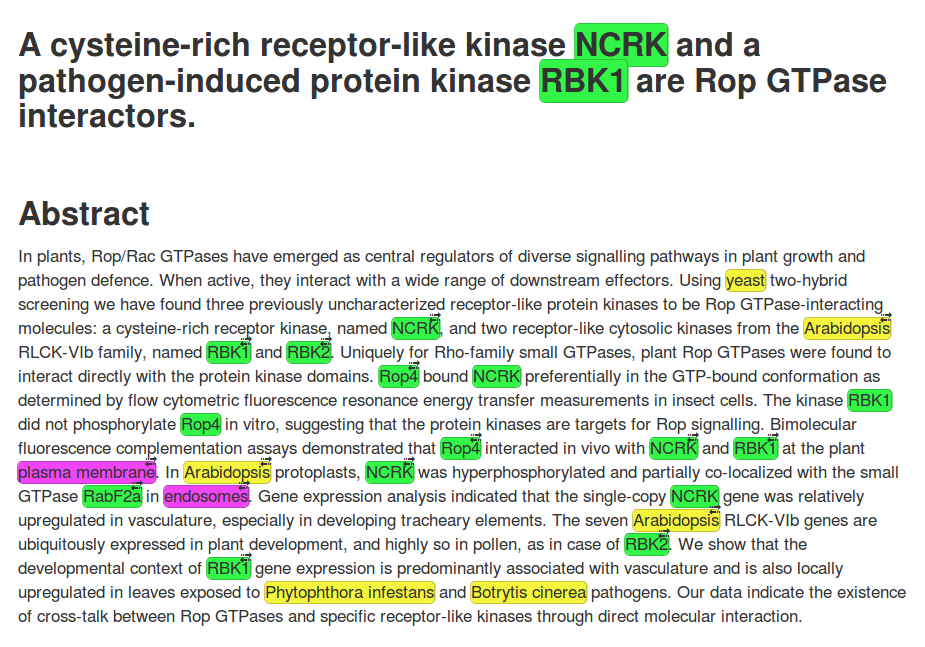
\includegraphics[scale=0.4]{figures/tagtog_screenshot.png}
\caption{Screenshot of an abstract from tagtog annotation tool}\label{fig:tagtogScreenshot}
\end{figure}

Figure \ref{fig:tagtogScreenshot} shows an example abstract annotated in tagtog annotation tool. The proteins, locations and organisms are highlighted in yellow, green and magenta respectively. The entities which participates in either protein-organism or protein-location relation, has a double arrow as an additional marking.

\section{Inter-annotator agreement (IAA)}

Inter-annotator agreement is a term quite often used in linguistics. It determines the agreement between different annotators on predefined set of documents. If the inter-annotator agreement is high, it implies that the annotation guidelines are very clear and different annotators agreed on most of the annotations.

As mentioned earlier, 46 out of 100 abstracts were used for developing annotation guidelines. The remaining 54 abstracts were independently annotated by me and my teammate Tatyana Goldberg using annotation guidelines. The inter-annotator agreement was calculated using annotations from these 54 abstracts. The inter-annotator agreement was denoted by F1 score and it was calculated separately for entity and relation annotations. The F1 score was calculated using following formula:

$$
F1 = \frac{2*X_{AB}*X_{BA}}{X_{AB}+X_{BA}}
$$

where $X_{ij}$ is the fraction of annotations by annotator i matching those of annotator j.

Since the focus of corpus annotation was protein-location relation extraction, the IAA was mainly calculated for annotations of entities, viz. proteins and subcellular locations and annotations of protein-location relations.

\subsection*{IAA for entities}

Two annotations of the same entity were considered to match if they have the exact same start offsets and end offsets. The IAA between two annotators was F1 score of  96\% and 88\% for protein and location annotations respectively. The combined F1 score for entity types was 94\%.

\subsection*{IAA for relations}

A protein-location relation annotation was defined to match between two annotators if annotations of both the protein and location entity match between the annotators, according to the definition above.

The IAA between two annotators was F1 score of 80\% for protein-location relations.

\section{Important insights from the corpus and publication of results}

% Explain about the results that you published at the BLAH conference
Some important insights were derived from LocText annotation. It was found out that the annotations in databases such as UniprotKB aren't complete and there is a room for improvement.

The results \cite{goldberg2015linked} were published in the symposium at Biomedical Linked Annotation Hackathon (BLAH) 2015 \cite{blah}. It was found out that since the biomedical research community and the natural language processing (NLP) community both undertake the annotations of text with different objectives in mind, linked annotations comprising of contributions from both communities could be immensely helpful. 

The annotation of corpus was done from scratch without actually referring to the annotations present in knowledge bases like UniProtKB. When the protein-location relations present in the corpus were compared with the information already present in the knowledge bases, it was found out that the corpus has more annotations for the same set of documents compared with UniProtKB.

The annotations in LocText were divided in three categories, viz. existing, more detailed and novel. Existing annotations are the ones that are present in knowledge bases already. The annotations were defined as more detailed annotation if they provide more information than what is present in the knowledge bases. In the same way, the annotations were defined as novel annotations if they are not present in the knowledge bases. The annotations were further subdivided based on whether or not the relationships involve UniprotKB proteins that cite the abstract.

\begin{table}
\centering
\begin{tabular}{|c|c|c|c|c|c|c|}
\hline
\textbf{Category} & \multicolumn{2}{c|}{\textbf{Existing}} & \multicolumn{2}{c|}{\textbf{More detailed}} & \multicolumn{2}{c|}{\textbf{Novel}} \\ 
\hline
\textbf{Citing Protein} & \textbf{Yes} & \textbf{No} & \textbf{Yes} & \textbf{No} & \textbf{Yes} & \textbf{No} \\
\hline
Human & 29 & 15 & 1 & 1 & 14 & 3 \\
Budding Yeast & 22 & 14 & 5 & 3 & 6 & 5 \\
Arabidopsis & 19 & 7 & 5 & 2 & 6 & 7 \\
Other & 2 & 9 & 0 & 0 & 0 & 6 \\
\hline
Subtotal & 72 & 45 & 11 & 6 & 26 & 41 \\
\hline
\textbf{Total} & \multicolumn{2}{c|}{\textbf{117}} & \multicolumn{2}{c|}{\textbf{17}} & \multicolumn{2}{c|}{\textbf{67}} \\ 
 \hline
\end{tabular}
\caption{Comparison of protein-location annotations in LocText with information available in UniProtKB}\label{tab:novelAnnotation}
\end{table}

% Write about observations from table here
As shown in the fig. \ref{tab:novelAnnotation}, novel or more detailed annotations could be found out for 84 out of 201 (42\%) proteins in 34 abstracts. For example, as seen in fig. \ref{fig:tagtogScreenshot}, the Arabidopsis protein RabF2a is localized to the endosomes which at the time of publication of results was not recorded in UniProtKB entry RAF2A\_ARATH.

From these results, it can be concluded that manually annotated corpora can contribute novel information about proteins in addition to what is present in the knowledge bases. Therefore, a case study was presented which proves that the creation of linked annotation resource would contain more annotations. In addition, the linked annotation resource would also create a synergy between biomedical research community and natural language processing community.

\section{Corpus statistics}\label{sec:corpusStats}

% Put all the numbers with respect to number of entities, relations and their distribution here. Also, put all the nice graphs that you made here

\subsection*{Count of entities and relations}

\begin{figure}
\centering
\begin{minipage}{.5\textwidth}
  \centering
  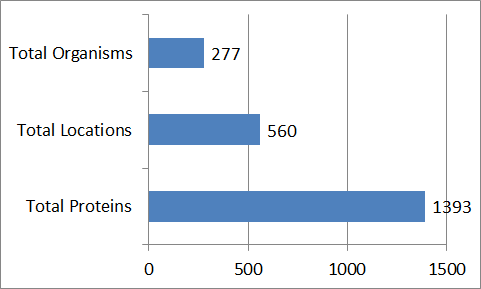
\includegraphics[width=.95\textwidth]{figures/ProtLocOrg_Distribution.png}
  \caption{Entities in LocText corpus}
  \label{fig:LocText_Entities}
\end{minipage}%
\begin{minipage}{.5\textwidth}
  \centering
  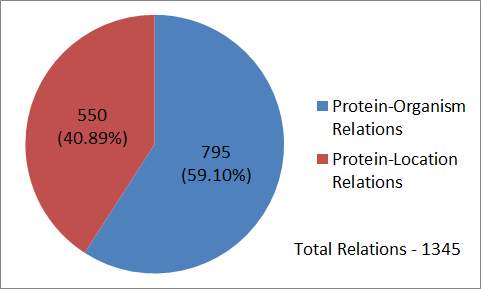
\includegraphics[width=.95\textwidth]{figures/AllRelationsPie.png}
  \caption{Relations in LocText Corpus}
  \label{fig:LocText_Relations}
\end{minipage}
\end{figure}

Fig. \ref{fig:LocText_Entities} and \ref{fig:LocText_Relations} shows the count of entities and relations present in 100 abstracts of LocText corpus. As shown in the fig. \ref{fig:LocText_Entities}, there are 1393 protein, 560 location and 277 organism annotations in the corpus. Similarly, fig. \ref{fig:LocText_Relations} shows that there are a total of 1395 relations in the corpus, 550 of which are protein-location relations and 795 are protein-organism relations. Protein-organism relations contributes nearly 60\% of the total relations whereas protein-location relations makes up remaining 40\%.

\subsection*{Analysis of relations}

\begin{figure}
\centering
\begin{minipage}{.5\textwidth}
  \centering
  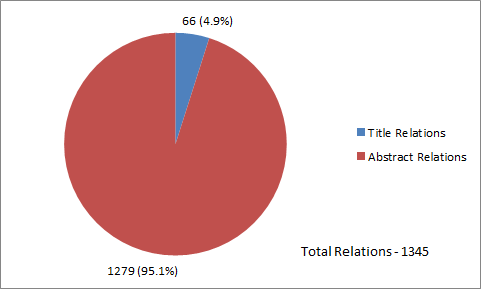
\includegraphics[width=.95\textwidth]{figures/Rel_Title_Abs_Distribution.png}
  \caption{Distribution in corpus}
  \label{fig:Rel_Title_Abs}
\end{minipage}%
\begin{minipage}{.5\textwidth}
  \centering
  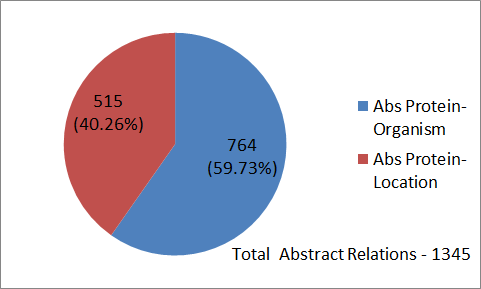
\includegraphics[width=.95\textwidth]{figures/AbsRel_PO_PL_Distribution.png}
  \caption{Distribution in abstract}
  \label{fig:Rel_Abs_PO_PL}
\end{minipage}
\end{figure}

We categorize the relations in two key categories, viz. same sentence relations and  different sentence relations. Same sentence relations are those relations in which both participating entities lie in the same sentence and different sentence relations are those relations in which either of the participating entities is in a different sentence. Same sentence relations can also be defined as intra sentence relations and different sentence relations can be defined as inter sentence relations.

The corpus is made by annotating 100 MEDLINE documents. Every document has a title and an abstract. The relations that are present in the title are all same sentence relations since there isn't a single document in the corpus where title spans more than one sentence.

As seen in the fig. \ref{fig:Rel_Title_Abs}, only a minor fraction (5\%) of relations are present in the title while remaining 95\% relations are present in the abstract. Morever, this also implies that the 5\% relations that are present in the title are all same sentence relations.

Fig. \ref{fig:Rel_Abs_PO_PL} shows the distribution of relations in the abstract according to its type. Of the total relations present in the abstracts, about 40\% are protein-location relations and about 60\% are protein-organism relations. Note that this distribution of protein-location and protein-organism relations is consistent with the distribution in the corpus as a whole (illustrated in fig. \ref{fig:LocText_Relations}).

\begin{figure}
\centering
\begin{minipage}{.5\textwidth}
  \centering
  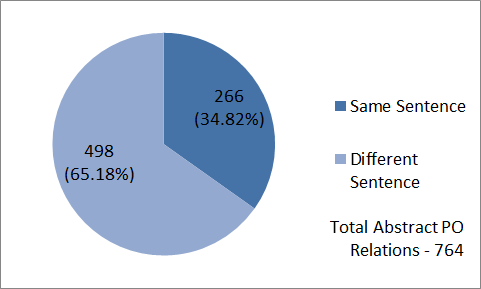
\includegraphics[width=.95\textwidth]{figures/AbsPORels_sent_Distribution.png}
  \caption{Abstract PO Relations}
  \label{fig:Abs_PO_Rel}
\end{minipage}%
\begin{minipage}{.5\textwidth}
  \centering
  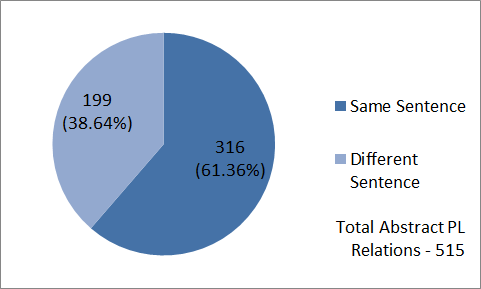
\includegraphics[width=.95\textwidth]{figures/AbsPLRels_sent_Distribution.png}
  \caption{Abstract PL Relations}
  \label{fig:Abs_PL_Rel}
\end{minipage}
\end{figure}


Fig. \ref{fig:Abs_PO_Rel} and \ref{fig:Abs_PL_Rel} shows the distribution of protein-organism (PO) and protein-location(PL) relations into same sentence relations and different sentence relations. As shown in fig. \ref{fig:Abs_PO_Rel}, about 35\% of the PO relations are same sentence relations and 65\% are different sentence relations. While in terms of PL relations, \ref{fig:Abs_PL_Rel} shows that about 61.4\% of the PL relations are same sentence relations and 38.6\% are different sentence relations.

\begin{figure}
\centering
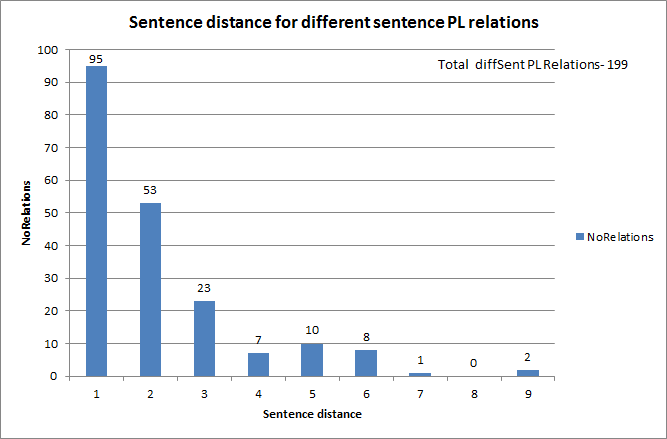
\includegraphics[scale=0.7]{figures/SentenceDistance_PLRel.png}
\caption{Sentence distance for PL Relations}\label{fig:SentDistancePL}
\end{figure}

The relations that are of prime interest are protein-location relations. From previous figures, it is already known that around 60\% of the PL relations in the abstract can be found in the same sentence. Fig. \ref{fig:SentDistancePL} shows how the PL relations which are different sentence relations are distributed according to the sentence distance. The different sentence relations in which the participating entities are in neighboring sentences is said to have a sentence distance of 1. In other words, the sentence distance of 1 indicates that the entities participating in the relation are 1 sentences apart. 

As seen in the fig. \ref{fig:SentDistancePL}, it is also possible to find the relations with sentence distance of 9 which means that the participating entities are 9 sentences apart. However, most of the different sentence relations have lower sentence distance. For example, about 95 out of 199 (47.74\%) different sentence relations are 1 sentences apart.

%TODO need a figure for distribution of PO PL in title as well.

Therefore to summarize the discussion, we come to the conclusion that 316/515 abstract PL relations (fig. \ref{fig:Abs_PL_Rel}) and 35 title PL relations are same sentence relations, which mean that about 351/550 (63.81\%) of total PL relations are same sentence relations. As seen from  fig. \ref{fig:SentDistancePL}, 95/199 (47.74\%) different sentence relations are at the distance of 1. Therefore, a total of 446/550 (81.09\%) PL relations are either same sentence relations or have a sentence distance of 1. This also implies that for about 81\% PL relations the participating entities are either in the same sentence or in the neighboring sentences. Hence, even if these 81\% relations could be extracted with high accuracy, it would be possible to extract a significant amount of information from the text.

\section{Linked annotation}

%Write about contribution in BLAH

\begin{figure}
\centering
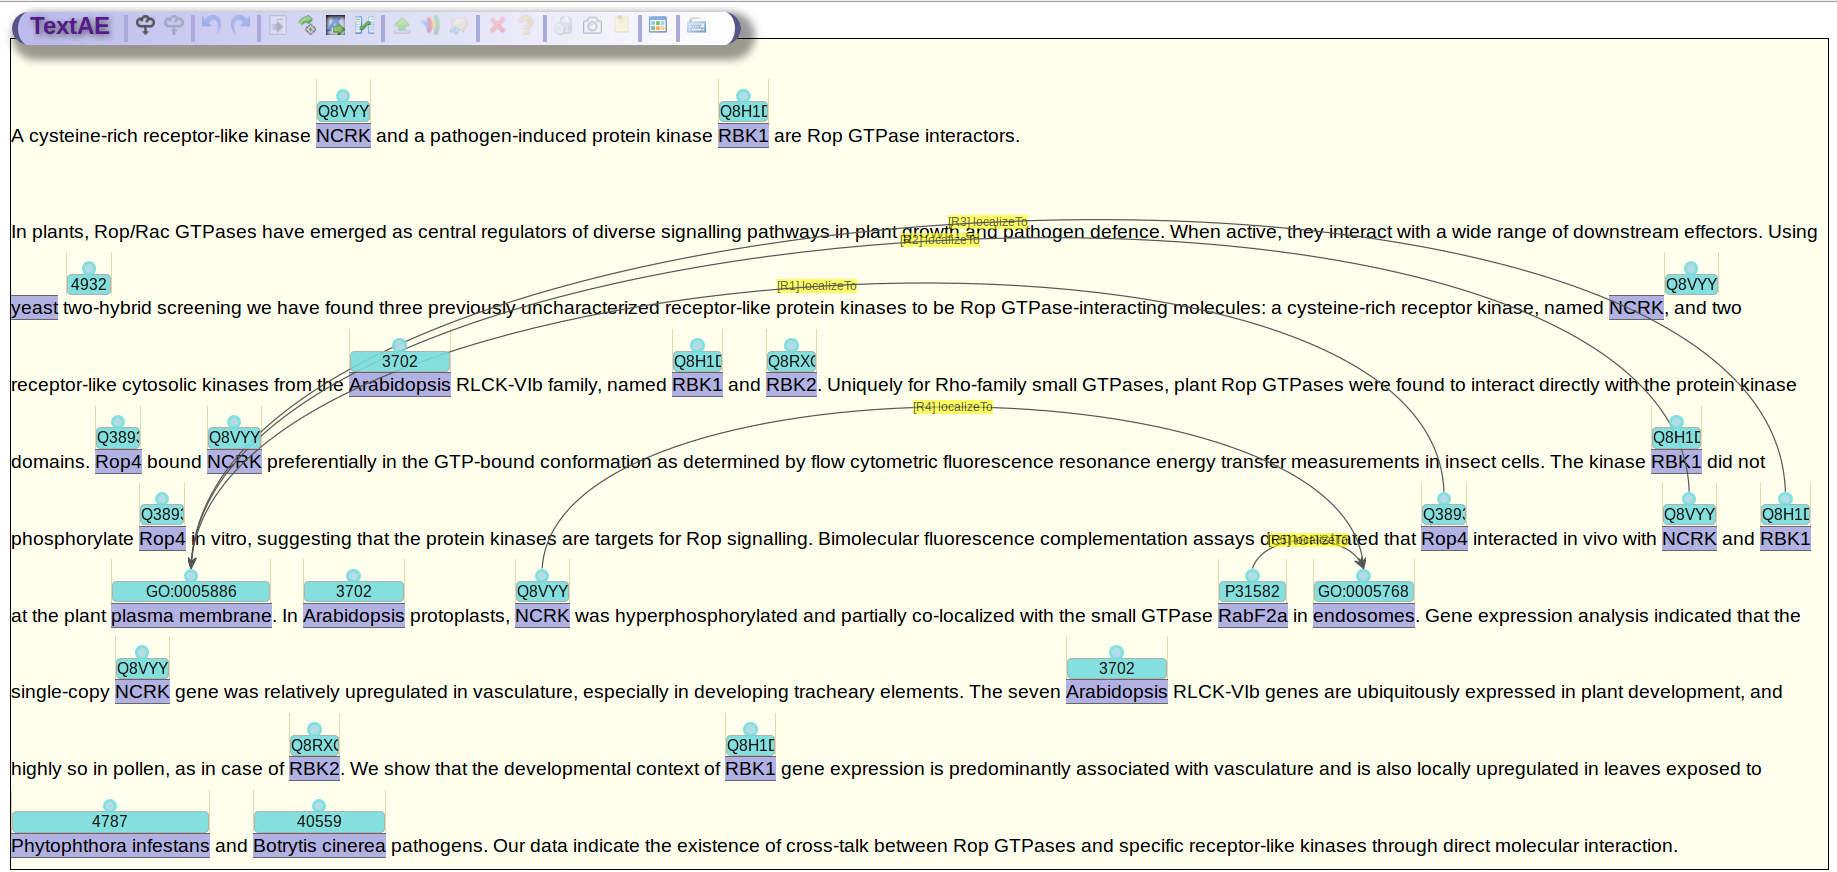
\includegraphics[scale=0.25]{figures/TextAE_Vis.png}
\caption{Visualization of annotations in TextAE}\label{fig:TextAEVis}
\end{figure}

As a part of the efforts to create a \hyperref[http://2015.linkedannotation.org/background]{linked annotation} resource, we also participated in the event BLAH \cite{blah} and the symposium. 

The tagtog annotation web interface stores the annotation in a different format than the format used at the BLAH hackathon. At the hackathon, the data was to be used in PubAnnotation format. PubAnnotation \cite{kim2012pubannotation} is a repository of text annotations and it has its own format to represent the annotation for any article. It also uses a visualization tool TextAE \cite{textae} for visualizing the annotations. Therefore, the data in tagtog JSON format was converted to PubAnnotation JSON format. The annotations which are shown in fig \ref{fig:tagtogScreenshot} are represented as fig. \ref{fig:TextAEVis} in the TextAE visualization tool. 

The LocText corpus is available for download under \hyperref[https://creativecommons.org/licenses/by/4.0/]{Creative Commons Attribution 4.0} in \hyperref[https://www.tagtog.net/-corpora/loctext]{tagtog} format and \hyperref[http://pubannotation.org/projects/LocText]{PubAnnotation} format.